\documentclass[dvips,ruledheader]{abnt}
\usepackage[brazil]{babel}
\usepackage[latin1]{inputenc}
\usepackage[pdftex]{graphicx}
% \usepackage[pdftex]{hyperref}
\usepackage{abnt-alf}
\usepackage{latexsym}
\usepackage{psfrag}
\usepackage[center]{caption2}
\usepackage{epigraph}

% Gloss�rio n�o utilizado
% \usepackage{makeglo}
% \renewcommand{\glossaryname}{Gloss�rio}
% \makeglossary

\begin{document}

\DeclareGraphicsRule{.eps.gz}{eps}{.eps.bb}{`gunzip -c #1}

% \begin{figure}[htp]
	\centering
	
\includegraphics[scale=1.5]{Figuras/capa}
% 	\caption{Tentativas de Fraudes Reportadas - 2012}
% 	\label{fig:estatisticas-fraudes-reportadas}
\end{figure}
\titulo{Workshop Cibercrime}

\autor{�lvaro Vilobaldo Rios da Silva (711605-1)\protect\\Douglas Botelho (71170847)\protect\\Marcio Fernandes Justino (7116006-1) }

\orientador[Professor]{Ant�nio Carlos Gesteira}

\comentario{Workshop de Cibercrime com foco em fraudes desenvolvido para a disciplina do 
2� Semestre de Fraudes Corporativas do Curso de P�s-Gradua��o em Computa��o Forense }

\instituicao{P�s-Gradua��o Lato Sensu em Computa��o Forense \par
Universidade Presbiteriana Mackenzie de S�o Paulo}

\local{S�o Paulo -- SP}

\data{\today}

\capa
\folhaderosto

\tableofcontents

\ 

\vfill

\begin{flushright}
\hfill \textit{Eles j� provaram que s�o sem escr�pulos. \\E se, um dia, uma rede terrorista resolver empreg�-los? \\(Igor Lopes - Jornalista) }
% 
% ``Man� j� nasce com o bolso da ca�a virada para baixo'' (Bezerra da Silva).
% Dedicamos esta disserta��o aos nossos pais,\\ cujo exemplo de honestidade e trabalho\\ nos marcaram as vidas,\\ e as nossas companheiras\\ que nos apoiaram nos momentos mais dif�ceis.}
\end{flushright}

\vspace*{1cm}

\clearpage
\chapter*{Introdu��o}

Esse documento � fruto dos estudos elaborados para o trabalho da disciplina do 2� Semestre de Fraudes Corporativas ministrado por Ant�nio Carlos Gesteira do Curso de P�s-Gradua��o Lato Sensu em Computa��o Forense da Universidade Presbiteriana Mackenzie de S�o Paulo. 

O que � cybercrime? Como combat�-lo? Como evit�-lo? Isso � poss�vel? Essas foram algumas das perguntas que nos fizemos durante o desenvolvimento desse trabalho e que condensamos nesse workshop vamos falar sobre os principais crimes praticados pelos meios eletr�nicos, contudo sendo um tema demasiado complexo e abrangente apresentando constantemente novas tecnologias e novas formas de opera��o do crime n�o ser� poss�vel mostrar tudo a respeito do mesmo.
\chapter*{Objetivo}

Este workshop tem por objetivo ampliar os conhecimentos sobre Cybercrime, dissertando sobre as fraudes praticadas, alguns casos reais, o modus operandi do criminoso, as preven��es, o processo de forense em Cybercrime e a forma de combate ao Cybercrime sempre embasando em fontes confi�veis para os dados apresentados. O workshop deve ser conclu��do at� o dia 20 de Junho de 2012, quando ser� entregue em meio digital, impresso e apresentado pelos seus integrantes.

\chapter{Cibercrime}

\epigraph{For hard cash, we will lie and deceive\\Even our masters don't know the web we weave} {Dogs Of War - Pink Floyd}

Segundo o livro \emph{Desvendando a Computa��o Forense} \cite{DCF2011}, existem dois tipos de crimes ligados aos computadores. No primeiro, o computador � uma ferramenta para a pr�tica do il�cito, como seria o papel ou caneta; j� o outro o computador � pr�prio meio do crime, ou seja, sem o mesmo o crime n�o poderia acontecer.

De acordo com \emph{Incident Response: Computer Forensics Toolkit} \cite{SCH2003} o \emph{Departamento de de Justi�a} norte americano prev� tr�s ocasi�es onde o crime se comuta com a computa��o, sendo eles, quando o computador � o alvo de ataque (virus, malware, invas�o, phishing), serve para armazenamento de dados crimosos (contabilidade de traficantes) e como ferramenta para cometer o delito (plano do crime num documento).

Como vimos, o departamento de justi�a norte americano ainda define mais uma forma do computador estar envolvido em atos il�citos a qual seria o armazenamento de dados crimosos como � o caso da contabilidade contida num arquivo do Excel\footnote{Microsoft Excel} referente ao tr�fico de drogas. Contudo ao armazenar informa��es no computador o mesmo estaria sendo usado como ferramenta.

J� a Wikip�dia \cite{WIKCI} define cybercrime da seguinte forma: 

\begin{citacao}
Crime inform�tico, e-crime, cybercrime, crimes eletr�nicos ou crime digital s�o termos utilizados para se referir a toda a atividade onde um computador ou uma rede de computadores � utilizada como uma ferramenta, uma base de ataque ou como meio de crime.
\end{citacao}

O que podemos afirmar com base nas refer�ncias e l�gicas mostradas acima � que cibercrime � todo crime que tem o computador ou redes como seu principal meio.

\section{Crimes de inform�tica mais comuns}

``Segundo o IPDI (Instituto de Peritos em Tecnologias Digitais e Telecomunica��es), pessoas que usam a inform�tica para roubar identidades podem responder por estelionato, furto mediante fraude, intercep��o de dados, quebra de sigilo banc�rio e forma��o de quadrilha.'' \cite{FLCC}

\begin{itemize}
  \item[$\bullet$]Roubo de Identidade: os internautas s�o enganados tendo sua identidade tomada para realiza��o de compras on-line, transfer�ncias financeiras indevidas, etc; 
  \item[$\bullet$]Pedofilia: cria��o de sites e/ou fornecimento/compartilhamento de material relacionado ao abuso sexual infantil; 
  \item[$\bullet$]Cal�nia e Difama��o: divulga��o de informa��es n�o ver�dicas, prejudiciais � v�tima. Muito comum nos sites de relacionamentos;
  \item[$\bullet$]Amea�a: e-mail, post em sites, com intuito amea�ador � v�tima; 
  \item[$\bullet$]Discrimina��o: divulga��o de conte�do relacionado ao preconceito - ra�a, religi�o, cor, etnia, proced�ncia. Tamb�m muito comum com o crescimento das redes sociais; 
  \item[$\bullet$]Fraudes; e
  \item[$\bullet$]Espionagem Industrial: aquisi��o de informa��o sigilosa de uma empresa por um concorrente. Com o avan�o tecnol�gico e a falta ou falha de controles de seguran�a, essa pr�tica tem se intensivado, sendo facilitada pela quantidade de informa��es que se pode carregar em um dispositivo m�vel.
\end{itemize}

\section{Fraudes}

Como pode ser observado nos estudos da CERT.br \cite{CERT} apresentado na figura \ref{fig:estatisticas-quadro-geral-incidentes}, a fraude � um dos incidentes com maior ocorr�ncia na atualidade.

\pagebreak

\begin{figure}[htp]
	\centering
	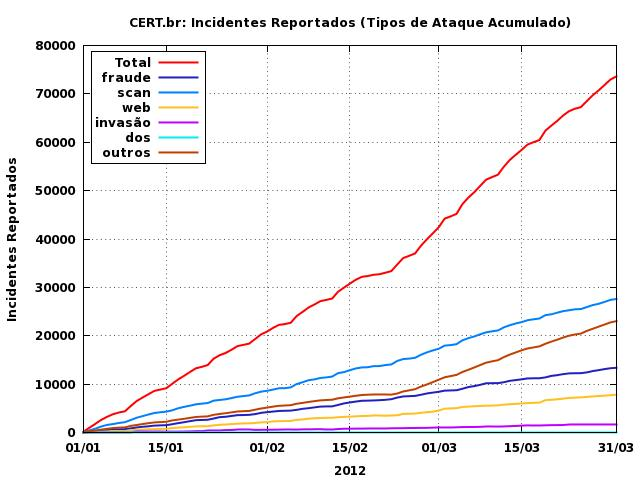
\includegraphics[scale=0.8]{Figuras/estatisticas-quadro-geral-incidentes}
	\caption{Incidentes Reportados - 2012}
	\label{fig:estatisticas-quadro-geral-incidentes}
\end{figure}

Dentro dos incidentes de fraude reportados pela \cite{CERT}, pode-se constatar que a utiliza��o de p�ginas falsas para ludibriar o usu�rio ocupa a maior faixa de ocorr�ncias, atingindo mais de 50\% dos incidentes, o que pode ser demonstrado na figura \ref{fig:estatisticas-fraudes-reportadas}.

\begin{figure}[htp]
	\centering
	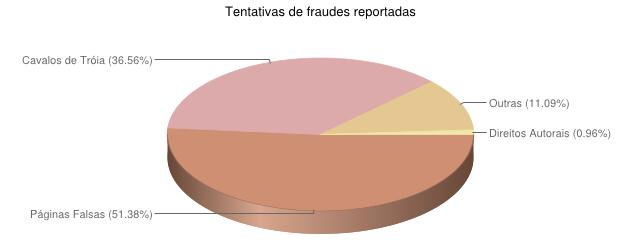
\includegraphics[scale=0.75]{Figuras/estatisticas-fraudes-reportadas}
	\caption{Tentativas de Fraudes Reportadas - 2012}
	\label{fig:estatisticas-fraudes-reportadas}
\end{figure}

\subsection{Agentes da Fraude}

Os agentes de fraudes podem ser de origem externa (o invasor sem confian�a) ou interna (funcion�rios com total confian�a pelos sistemas da corpora��o). Algumas fraudes mais elaboradas apresentam a participa��o de ambos agentes, sendo esta uma das formas mais utilizadas por organiza��es criminosas.

Dentro das fraudes cometidas por agentes internos, quando em cargos de chefia, pode-se destacar o preju�zo acentuado causado � organiza��o tendo visto em muitas vezes a falta de puni��o. \cite[p.~18-20]{GIL}.

\begin{figure}[htp]
	\centering
	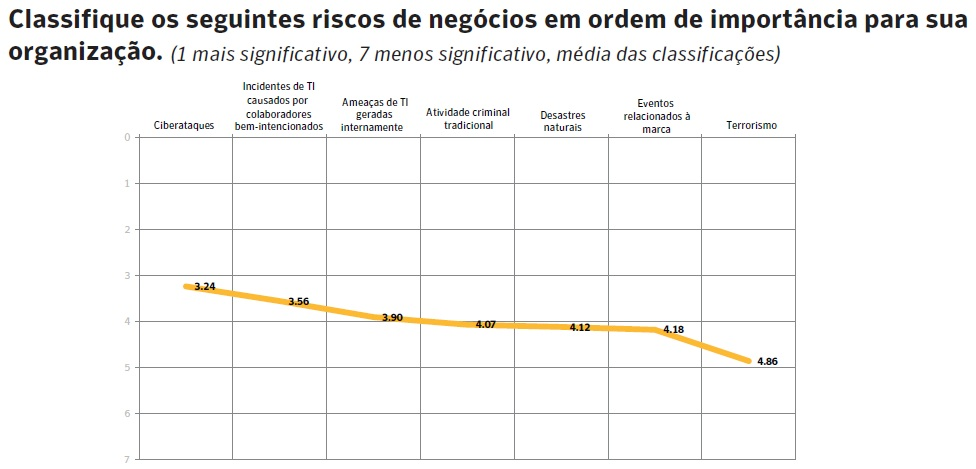
\includegraphics[scale=0.6]{Figuras/riscos-em-ordem-de-importancia}
	\caption{Riscos de neg�cios em ordem de import�ncia para a organiza��o\cite{SYMANTECREL2011}}
	\label{fig:riscos-em-ordem-de-importancia}
\end{figure}

Como mostra o relat�rio de seguran�a da Symantec\footnote{\cite{SYMANTECREL2011}}, os incidentes de seguran�a causados por cibercrime e por agentes internos s�o considerados os de maior risco para as organiza��es. Assim como as amea�as mais significantes est�o por conta da a��o dos hackers, ou agentes externos.

\begin{figure}[htp]
	\centering
	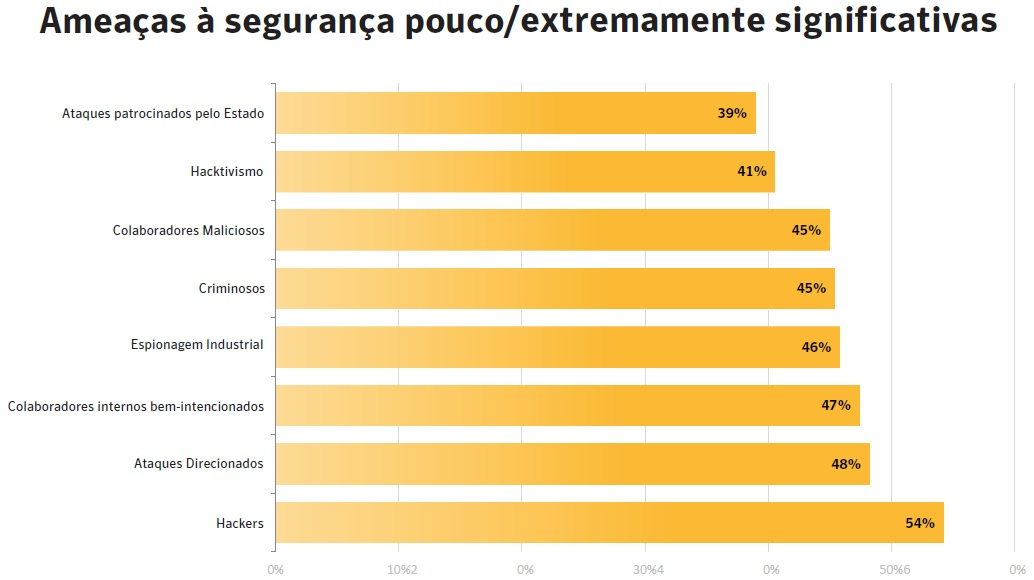
\includegraphics[scale=0.5]{Figuras/ameacas-significantes}
	\caption{Amea�as � seguran�a pouco/extremamente significativas \cite{SYMANTECREL2011}}
	\label{fig:ameacas-significantes}
\end{figure}

\section{Cibercrime Brasileiro}

O e-crime est� cada vez mais envolvido com o crime convencional, ``geralmente alimenta outros crimes, como o narcotr�fico'', ressalta F�bio Assonlini, analista de malware da Kaspersky no Brasil. 

O Brasil lidera o ranking com maior n�mero de bankers do mundo. No Brasil o cibercrimosos envolvidos com o roubo de dados banc�rios e clone de cart�es ficou conhecido como ``Raul'' \cite{ADCC}. Os crimosos se vangloriam e exp�em suas conquistas na pr�pria internet, onde temos diversos exemplos de m�sicas que at� mostram do modus operandi da coleta dos dados at� a melhor forma de utiliza��o \cite{FUNK}. Os brasileiros foram os primeiros a criarem um banker rootkit para arquitetura x64 (64 bit).

\subsection{Perfil do Banker Brasileiro}

Em geral o perfil do banker brasileiro � jovem, de baixa renda, que obt�m c�digos maliciosos de outros (Figura \ref{fig:CompraBot01}) para aplicar seus golpes.

\begin{figure}[htp]
	\centering
	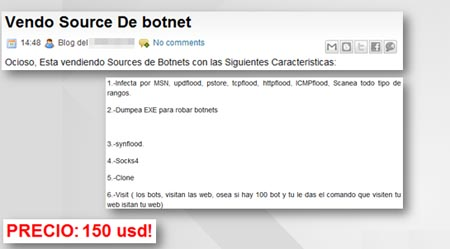
\includegraphics[scale=1]{Figuras/CompraBot01}
	\caption{An�ncio de botnet \cite{KAS}}
	\label{fig:CompraBot01}
\end{figure}

\pagebreak

Existem sites de comercializa��o de c�digos maliciosos espalhados pela internet, e alguns inclusive com direito a reclama��es de n�o entrega dos produtos (Figura \ref{fig:CompraBot02}).

\begin{figure}[htp]
	\centering
	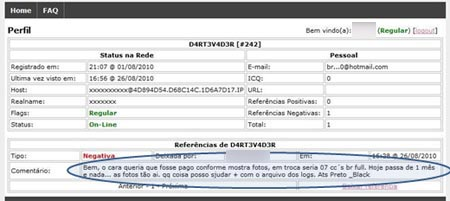
\includegraphics[scale=1]{Figuras/CompraBot02}
	\caption{"Procon" do site de vendas \cite{KAS}}
	\label{fig:CompraBot02}
\end{figure}

Outro assunto pertinente e curioso a respeito do cibercrime brasileiros � que para come�ar na vida crimosa virtual com maior conforto e menos esfor�o existem at� cursos onlines que ensinam atacar sites financeiros e a mandar spam \cite{SWKK}.
\chapter{Arquitetura Tecnol�gica}

Pela pr�pria natureza do cibercrime ser diversa e abrangente, os equipamentos utilizados para a sua pr�tica s�o t�o diversos e amplos quanto. Mesmo que os computadores sejam o principal meio, nada impede que tablets, smartphones, roteadores etc sejam utilizados de alguma forma como meio para cometer o crime cibern�tico. 

De forma an�loga as tecnologias empregadas pelos equipamentos ou dispon�veis para estes tamb�m s�o abrangentes. Segundo an�lises da Kaspersky Lab \cite{KAS} � comum uma especializa��o de c�digos maliciosos por regi�o. Nos EUA o c�digo malicioso mais comum s�o do tipo FAKEAV\footnote{Falsos antivirus}, na Europa oriental, Russia e pa�ses ib�ricos s�o mais comuns rootkits, o Brasil entretando se especializou na produ��o de c�digos maliciosos para furto de dados banc�rios e clones de cart�o de cr�ditos tamb�m conhecidos como bankers.

Como j� foi dito o Brasil foi classificado como pa�s l�der em v�rus que roubam dados banc�rios, tamb�m conhecido como trojans bankers, segundo pesquisa da Kaspersky Lab \cite{DWKS}, sendo o mesmo o 95\% dos c�digos maliciosos desenvolvidos no Brasil s�o justamente para esse intuito \cite{ADBV}.
\chapter{Abordagem Metodol�gica}

Existem v�rias modalidades de criminosos digitais. A maioria dos ataques (\~= 95\%) � proveniente de pessoas com pouco conhecimento em atividades Hacker.

As mais comuns fraudes da atualidade s�o origin�rias de Phishing - tipo de fraude projetada para roubar informa��es valiosas particulares. O phishing, comumente chamado de phishing scam ou scam, utiliza-se de pretextos enganosos para obter de sua v�tima informa��es relevantes tais como n�meros de cart�es de cr�dito, senhas, dados de contas, entre outros.

Para que o phishing funcione, o usu�rio mal-intencionado envia milh�es de emails falsos que parecem vir de sites populares ou de sites nos quais se tem confian�a, como site de uma institui��o financeira ou de uma empresa de cart�o de cr�dito. Esses emails, e os sites a que remetem, parecem oficiais o suficiente para convencer muitas pessoas de sua legitimidade. Acreditando que esses emails s�o leg�timos, pessoas desavisadas com frequ�ncia respondem �s solicita��es de recadastros, n�mero do cart�o de cr�dito, senha, informa��es de conta ou outras informa��es pessoais.

Para fazer com que esses emails pare�am ainda mais reais, os criadores de scams podem colocar um link em um email falso que parece levar ao site leg�timo, mas na verdade leva voc� ao site de scam ou mesmo a uma janela pop-up muito semelhante ao site oficial. Uma vez entrando em um desses sites, a v�tima poder�, inadvertidamente, inserir informa��es pessoais, que ser�o transmitidas diretamente ao criador do site. Ele poder� usar esses dados para comprar bens, candidatar-se a um novo cart�o de cr�dito ou roubar a identidade da v�tima.

\section{Caso Carolina Dieckmann}

Um caso exemplar de phishing que ganhou a m�dia nos �ltimos meses foi o caso da Carolina Dieckmann. No famigerado caso a atriz Carolina Dieckmann recebeu um spam solicitando o usu�rio e senha da sua conta de e-mail. Ao informar o dados a mesma concedeu acesso a sua conta do Gmail pelo qual a mesma havia enviados diversas fotos nuas e que ainda estavam armazenadas nos \emph{enviados}. Com as fotos em m�os os invasores chantagearam a atriz.

Veja a baixo um infogr�fico do caso.

\begin{figure}[htp]
	\centering
	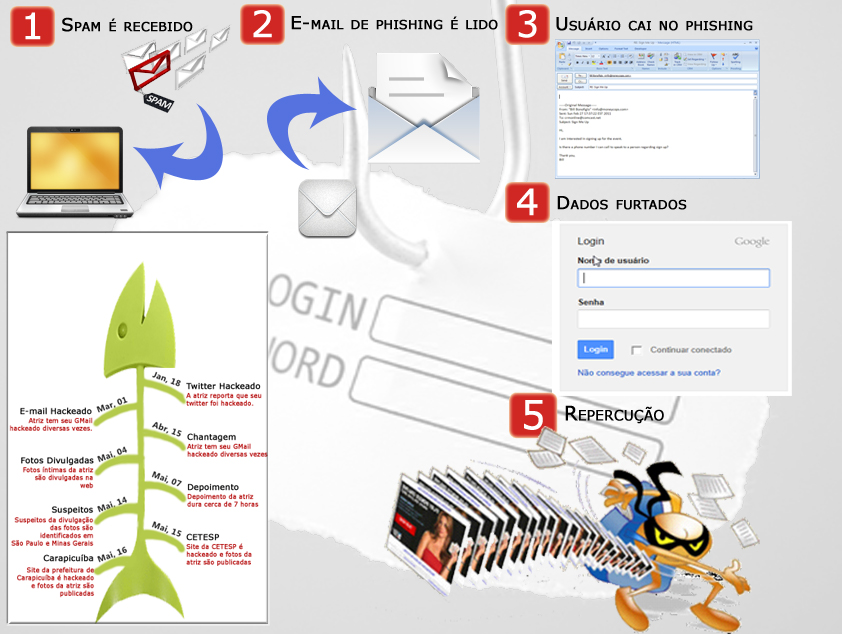
\includegraphics[scale=0.6, angle=90]{Figuras/info-caso-dieckmann01}
	\caption{Infogr�fico de um phishing scam}
	\label{fig:info-caso-dieckmann01}
\end{figure}


\section{Modus Operandi}

De maneira geral, o modus operandi � o comportamento necess�rio para a pr�tica de um crime com sucesso. No m�nimo, todo modos operandi deve envolver:

\begin{enumerate}
  \item Assegurar o sucesso do crime;
  \item Prote��o da identidade; e
  \item Fuga efeito.
\end{enumerate}

N�o se podem vincular casos pelo modus operandi, pois, o modus operandi � din�mico, mudando com a experi�ncia de a��o do criminoso. O aprendizado comportamental � como qualquer outro. Envolve maturidade, experi�ncia e instru��o.

\begin{citacao}
Hackers tem encontrado uma forma de otimizar a efici�ncia da metodologia cl�ssica ou do livro de receitas (cook-books). Os desenvolvimentos mais recentes mostram o uso de v�rus e trojans como parte do modus operandi (Richard Stiennon da IT-Harverst).
\end{citacao}

As figuras \ref{fig:anatomyhackold} e \ref{fig:anatomyhacknew} demonstram a anatomia hacker, como era e como � atualmente.

\begin{figure}[htp]
  \centering
  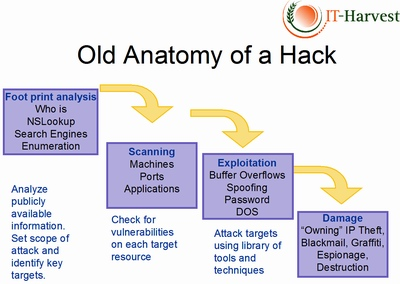
\includegraphics[scale=0.8]{Figuras/anatomyhackold}
  \caption{Antiga anatomia hacker \cite{MODUSOPE}}
  \label{fig:anatomyhackold}
\end{figure}

\pagebreak

\begin{figure}[htp]
  \centering
  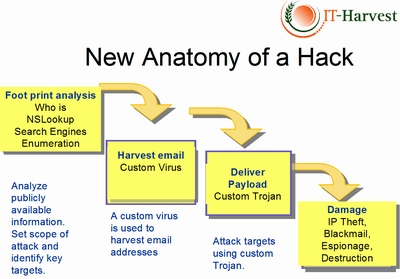
\includegraphics[scale=0.8]{Figuras/anatomyhacknew}
  \caption{Nova anatomia hacker \cite{MODUSOPE}}
  \label{fig:anatomyhacknew}
\end{figure}

A diferen�a entre elas � que na nova anatomia o hacker se utiliza de v�rus e trojans, desenvolvidos de forma costumizada, tendo este o mesmo efeito de algu�m se infiltrar e instalar um keylogger ou um keystroke logger na m�quina alvo. O novo m�todo � considerado mais f�cil e mais abrangente que o m�todo antigo.

\section{Estrutura do crime}

Como foi analisado acima a anatomia dos ataques vai se modificando com o tempo. De forma parecida a estrutura para se cometer crimes online tamb�m evoluiu.

Antigamento o desenvolvedor do c�digo malicioso era o mesmo que o disseminava e o que tinha a conta banc�ria preenchida com o montade dos furtos. Contudo essa abordagem se mostrou fr�gil e facilmente rastre�vel.

Hoje o crime trabalha de forma bem estruturada e especializada. Veja abaixo:

\begin{enumerate}
  \item O desenvolvedor de c�digos maliciosos apenas vende ou repassa gratuitamente o c�digo;
  \item O crimoso utiliza o c�digo malicioso para capturar dados das vitimas por meio de spams e sites falsos;
  \item O aliciador recruta laranjas para despistar o rumo do dinheiro furtado; e
  \item O laranja fica na base desse piramide, sendo ele a posi��o mais delicada e perigosa.
\end{enumerate}

\subsection{Laranjas}

\epigraph{Esse cara � um acerola, pois vale por 10 laranjas} {Domingo Montanaro}

No mundo do crime organizado existem dois tipos de laranja: o pessoa f�sica e o pessoa jur�dica.

No primeiro caso as pessoas s�o aliciadas para receberem montantes de dinheiro direto em suas contas banc�rias e ent�o fazerem transfer�ncias desse dinheiro para outras contas (que podem ser de laranjas). Em geral o laranja � aliciado por an�ncios espalhados em sites legitimos como ``Ganhe dinheiro sem sair de casa'' (Figura \ref{fig:ganhe_dinheiro}) embolsando de 5\% a 10\% do valor furtado.

\begin{figure}[htp]
	\centering
	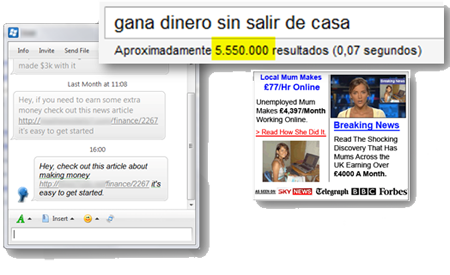
\includegraphics[scale=1]{Figuras/ganhe_dinheiro}
	\caption{An�ncio para pegar laranjas\cite{KAS}}
	\label{fig:ganhe_dinheiro}
\end{figure}

Muitas vezes o laranja � o �nico a ir preso j� que o mesmo n�o tem ideia de como funciona a cadeia crimosa e existem casos que ele nem sabe que faz parte de uma cadeia crimosa e � aliciado crendo que participa de uma atividade legal.

O laranja pessoa jur�dica os criminosos abrem uma empresa e usam os cart�es clonados pelos bankers e carders para comprar produtos e os vendem em lojas desconhecidas por pre�os muito a baixo do mercado, faturando e lavando o dinheiro no processo.
\chapter{Preven��o}

A preven��o visa impedir e ou inibir a��es criminosas aos sistemas, tendo visibilidade maior onde o dano causado pode ser maior.
A prote��o se baseia em \cite[p.~545-546]{TURBAN}:

\begin{itemize}
	\item[$\bullet$]Preven��o;
	\item[$\bullet$]Deten��o;
	\item[$\bullet$]Detec��o;
	\item[$\bullet$]Limita��o;
	\item[$\bullet$]Recupera��o; e
	\item[$\bullet$]Corre��o.
\end{itemize}

� necess�rio agir preventivamente nesses pontos de atua��o criminosa. Sistemas com fraca autentica��o, o compartilhamento de senhas, a falta de rastreabilidade e vulnerabilidades de conectividade e mobilidade s�o os maiores motivadores para ocorr�ncias de Cibercrime.

Existem diversas for�as preventivas que inibem o ato criminoso digital, entre elas:

\begin{itemize}
	\item[$\bullet$]Gest�o de perfis;
	\item[$\bullet$]Monitoramento;
	\item[$\bullet$]Autentica��o forte;
	\item[$\bullet$]Fortalecimento dos sistemas;
	\item[$\bullet$]Auditorias; e
	\item[$\bullet$]Fator Humano.
\end{itemize}

\begin{citacao}
Uma an�lise de custo-benef�cio mensurando a probabilidade de danos e perdas prov�veis que poderiam ser combatidas com a implanta��o de um sistema de preven��o de fraudes deve ser considerada \cite{FRAUELE}.
\end{citacao}

Alguns �rg�os, tais como o FBI, disponibilizam dicas para evitar fraudes e tamb�m setores para combater fraudes cibern�ticas \cite{IC3}.
Essas dicas podem ser encontradas online dispon�veis a todos que desejarem visualiz�-las.

Tamb�m est� dispon�vel online um servi�o para auxiliar na preven��o e combate a fraudes cibern�ticas, o Monitor das Fraudes \cite{MONITORFRAUDES} disponibiliza informa��es para identifica��o de fraudes, um dec�logo antifraudes com dicas e sugest�es para preven��o das mesmas.

\begin{figure}[htp]
	\centering
	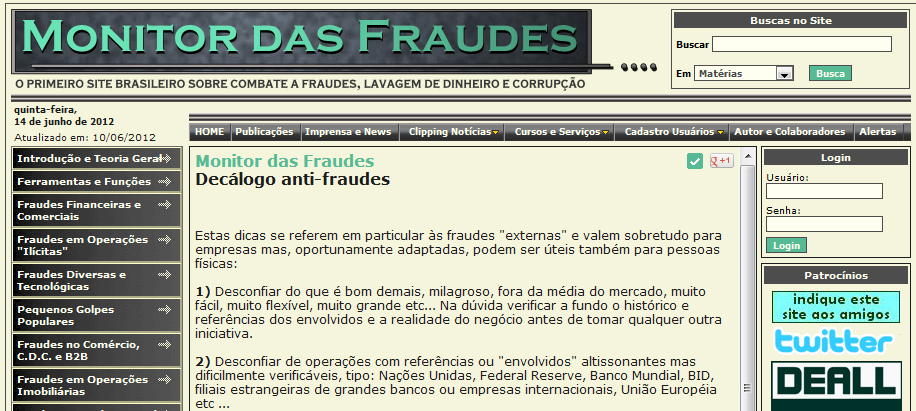
\includegraphics[scale=0.5]{Figuras/prevencao-monitor-das-fraudes}
	\caption{\cite{MONITORFRAUDES}}
	\label{fig:prevencao-monitor-das-fraudes}
\end{figure}

Existem atualmente in�meras solu��es que auxiliam na preven��o e no combate a fraudes cibern�ticas. AntiSpams, AntiVirus, Firewalls, Controle de Acesso (Biometria, Leitura �tica, etc.), Certificados Digitais.

\section{Normas de Seguran�a}

Diversos padr�es foram desenvolvidos para melhorar a seguran�a das organiza��es, prevenindo e preparando a mesma para reagir ao incidente de forma coexa e r�pida evitando ao m�ximo as perdas de ativos e de capital.

Inclusive em determinadas �reas as empresas devem est� em conformidade a esses padr�es, como � o caso do PCI\footnote{Payment Card Industry\cite{PCI}} para empresas que lidam com transa��es de cart�o de cr�dito.

As normas da familia ISO 27000\footnote{\cite{ISO27000}} foram desenvolvidas para abranger a seguran�a da informa��o como um todo e unificar boas pr�ticas em um compilado em forma de normas guias. J� o COBIT\footnote{\cite{COBIT}} � um guia de boas pr�ticas em forma de framework para gest�o de TI.

� importante ressaltar que o em muitos casos a conformidade com as normas padr�es da �rea n�o s�o obrigat�rias, contudo s�o altamente recomendados e evitam ou atenuam diversas falhas ou quebras de seguran�a.

Como essas boas pr�ticas foram feitas para otimizar o trabalho dos gestores, auditores e analistas de seguran�a, os mesmos quando bem implentados criam um ambiente fortimente protegido e com ampla capacidade de resposta a incidentes, mesmo que seja imposs�vel garantir seguran�a total.

No �mbito forense as normas podem ajudar ao per�to, assist�nte t�cnico ou investigador a localizar desvios de conduta de funcion�rio ou encontrar eventos anormais no funcionamento de uma organiza��o diminuindo o tempo e os recursos gastos para a a��o.

\section{Novos Desafios}

Segue uma listas dos novos desafios:

\begin{itemize}
	\item[$\bullet$]Inova��o tecnol�gica.
	\item[$\bullet$]Engenharia social como fator humano.
	\item[$\bullet$]T�cnicas avan�adas de anti-forense e de evas�o.
	\item[$\bullet$]Legisla��o.
	\item[$\bullet$]Colabora��o internacional.
\end{itemize}

\subsection{Inova��o Tecnol�gica}
Devido � grande velocidade da evolu��o tecnol�gica, de m�dias, de dispositivos, de softwares e da pr�pria velocidade da internet e inclus�o digital, a tecnologia tem se tornado um grande desafio para os respons�veis pela seguran�a da informa��o.

\subsection{Engenharia Social}
Acompanhando a tecnologia, um outro fator que sempre tem sido um grande desafio, com a facilidade de acesso �s informa��es que � disponibilizada atualmente, o fator humado tamb�m � considerado como um grande desafio para a seguran�a da informa��o, tendo em vista ainda que sua fragilidade � utilizada em larga escala atualmente pelos cibercriminosos.

\subsection{T�cnicas Anti-Forense e de Evas�o}
As t�cnicas de anti-forense e de evas�o cada vez mais avan�adas, o uso de esteganografias, criptografia, etc.

\subsection{Legisla��o}
Necessidade de ajustes na legisla��o vigente para tipificar de melhor forma os crimes cibern�ticos.

\subsection{Colabora��o Internacional}
Colabora��o e coopera��o entre os �rg�os de preven��o e combate aos crimes cibern�ticos, agilizando os processos investigativos, mitigando a impunidade e a ocorrencia de novos incidentes.
\chapter{Quest�es Legais}

Hoje no Brasil n�o existe legisla��o espec�fica para cibercrimes. Ent�o os casos s�o tratados de modo geral pelo c�digo penal\footnote{\cite{CODPENAL}} vigente de 1940 que n�o tinha condi��es de prev� os avan�os tecnol�gicos que temos hoje tornando a tipica��o dos crimes confusa e divergente.

O crime digital n�o � inpun�vel no Brasil, pelo contr�rio, mesmo sendo tendo uma legisla��o antiga datada da d�cada de quarenta a mesma � gen�rica e ampla o suficiente para enquadrar em seus artigos muitos dos atos il�citos cometidos por meios eletr�nicos.

O crime digital pode acarretar em penas mais brandas do que os seus an�logos n�o digitais. No caso de um assalto a banco o que o faz pessoalmente o assaltante � enquadrado em roubo com pena de quatro a dez anos al�m de poder imputar-lhe agravante de que pode aumentar a pena pela metade j� a mesma quantidade de dinheiro roubado digitalmente incorre em furto simples onde a pena � de um a quatro anos e multa, j� que ningu�m pode ``Subtrair coisa m�vel alheia, para si ou para outrem, mediante grave amea�a ou viol�ncia a pessoa''\footnote{Art. 157 do C�digo Penal Brasileiro} de um computador.

Para remediar isso existem alguns projetos de lei (PL) que pretendem suprir essa necessidade, como � o caso da PL 2793/11\footnote{\cite{PL27903}} que ``Disp�e sobre a tipifica��o criminal de delitos inform�ticos; altera o Decreto-Lei n� 2.848, de 7 de dezembro de 1940 - C�digo Penal; e d� outras provid�ncias.'' que determina dentre outras coisas a pena de 3 meses a 1 ano pela invas�o de computadores para obter, adulterar ou destruir dados que at� a reda��o desse texto n�o tinha sido aprovada no senado. Al�m da famigerada Lei Azeredo\footnote{\cite{PL84}} que tamb�m ficou conhecido AI-5 digital por artigos confusos e amplos em demasia.
% \chapter{Forense}

\section{Investiga��o}

\subsection{Processo Legal}

\subsection{Como Investigar}

\subsection{Rastreabilidade}

\begin{itemize}
  \item[$\bullet$]Falhas cometidas pelos criminosos;
  \item[$\bullet$]Rastros deixados;
  \item[$\bullet$]Sistemas de rastreamento de invas�o;
\end{itemize} At� aqui revisado
\chapter{Combate}

\begin{citacao}
N�o h� como combater as fraudes eletr�nicas com efici�ncia sem comprometimento efetivo de provedores de internet, de email e de conte�do, lan houses, cyber caf�s e empresas de telecom, integrados em uma rede que deve reunir empresas, pessoas, autoridades e infraestrutura da sociedade digital \cite{PARTNERSALES}.
\end{citacao}

Alguns �rg�os contribuem no combate ao crime cibern�tico, reportando incidentes de seguran�a ocorridos.
Um desses �rg�os � o CAIS - Centro de Atendimento a Incidentes de Seguran�a. O mesmo tem a fun��o informativa e educativa, exibe uma cole��o de imagens de phishing scam e ou malwares veiculados por meio de spam.

�rg�os Nacionais que visam o combate do cibercrime:

\begin{itemize}
	\item[$\bullet$]Minist�rio P�blico Federal (MPF);
	\item[$\bullet$]Policia Civil;
	\item[$\bullet$]DIG-DEIC - 4� Delegacia de Repress�o a Crimes de Inform�tica de S�o Paulo (SP);
	\item[$\bullet$]DERCIFE (Delegacia Especializada de Repress�o a Crimes contra Inform�tica e Fraudes Eletr�nicas), em Belo Horizonte (MG); 
	\item[$\bullet$]DRCI - Delegacia de Repress�o aos Crimes de Inform�tica, no Rio de Janeiro (RJ), dentre outros. 
	\item[$\bullet$]Policia Federal;
	\item[$\bullet$]Ccomgex - Centro de Comunica��es e Guerra Eletr�nica do Ex�rcito;
	\item[$\bullet$]SaferNet: Iniciativa privada;
	\item[$\bullet$]Centro de Monitoramento do Servi�o de Repress�o a Crimes Cibern�ticos: Inicialmente criado para combater crimes financeiros realizados pela rede, o centro foi ampliado para tratar das tentativas e ataques a sistemas de informa��o do governo federal \footnote{\cite{RIO20}};
	\item[$\bullet$]Comiss�o de Direito eletr�nico e crimes de alta tecnologia da OAB de SP;
	\item[$\bullet$]CDCiber - Centro de Defesa Cibern�tica; e
	\item[$\bullet$]CAIS - Centro de Atendimento a Incidentes de Seguran�a.	
\end{itemize}

O combate ao cibercrime foi incorporado a �rg�os no mundo inteiro, podemos citar com destaques em �mbito internacional:

\begin{itemize}
	\item[$\bullet$]FBI (IC3 - Internet Crime Compliant Center); e
	\item[$\bullet$]Interpol.
\end{itemize}

Independente do �rg�o respons�vel, � bom salientar que o combate ao cibercrime deve vir a n�vel de Estado, tomando medidas como por exemplo:

\begin{itemize}
  \item[$\bullet$]Pol�ticas governamentais: legisla��o, pol�cias especializadas, departamentos de investiga��o etc;
  \item[$\bullet$]Coopera��o entre �rg�os;
  \item[$\bullet$]Ferramentas; e
  \item[$\bullet$]Informa��o: divulga��o de informa��es entre as pessoas e presen�a da m�dia.
\end{itemize}
\chapter{Vis�o de Produtos}
Atualmente existem diversas solu��es no mercado voltadas diretamente ou indiretamente � preven��o, combate ou conten��o de crimes realizados por meios digitais. Abaixo est�o dispostas algumas dessas solu��es para prote��o e descontamina��o de ambientes, controle de transa��es (e-commerce) e lavagem de dinheiro.

\section{Solu��es para Prote��o/Descontamina��o de Ambiente}
Os softwares encontrados s�o os softwares mais utilizados na atualidade e em geral possuem um \emph{``know-how''} e protegem os clientes com uma gama de sistemas especializados integrados \footnote{anti-virus, firewall, anti-spyware, etc} em uma solu��o completa.

\begin{itemize}
	\item[$\bullet$]F-Security;
	\item[$\bullet$]Kaspersky;
	\item[$\bullet$]McAfee;
	\item[$\bullet$]Symantec;
	\item[$\bullet$]ESET; e
	\item[$\bullet$]CheckPoint.
\end{itemize}

Em geral, apesar dos softwares apresentarem diferentes fabricantes, ambos oferecem servi�os similares de forma an�loga e qualidade razo�vel.

\section{Seguran�a de Transa��es (e-commerce)}

Esses sistemas visam maior controle transacional entre o cliente e o e-commerce, oferecendo garantias para ambas as pontas.

\begin{itemize}
	\item[$\bullet$]SuperPay
	\item[$\bullet$]Paypal;
	\item[$\bullet$]CelarSafe;
	\item[$\bullet$]Mercado Pago;
\end{itemize}

\section{Outros}

O setor de anti-fraude � muito criativo e diariamente surgem diversas solu��es ou pretensas solu��es que visam a resolu��o de diversas fontes de fraudes, como por exemplo o \emph{Wolters Kluwer - Banking Risk} com a promessa de evitar fraudes dentro da corpora��o \cite{TOOLKIT}.

\section{Detalhe de Ferramentas}

\subsection{Symantec Endpoint Protection}

\begin{figure}[htp]
	\centering
	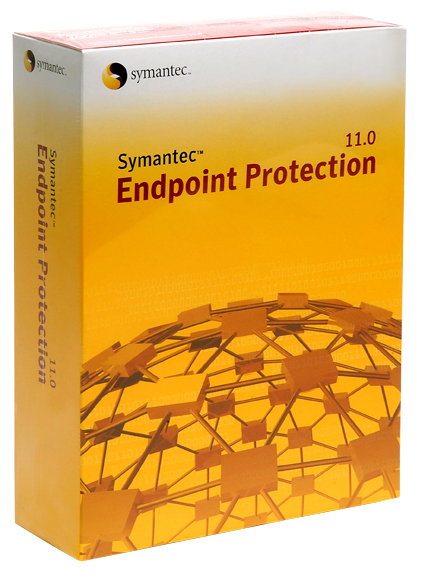
\includegraphics[scale=0.5]{Figuras/capa-symantec}
	\caption{Sysmantec Endpoint Protection \cite{SYMANTEC}}
	\label{fig:capa-symantec}
\end{figure}

O Symantec Endpoint \cite{SYMANTEC} Protection 12 combina o Symantec AntiVirus com uma  preven��o avan�ada contra amea�as, visando fornecer uma defesa inigual�vel contra malware para laptops, desktops e servidores. Ele integra perfeitamente tecnologias de seguran�a essenciais em um �nico agente e console de gerenciamento, o que aumenta a prote��o e ajuda a reduzir o custo total de propriedade.

Principais benef�cios:
\begin{itemize}
	\item[$\bullet$]Bloqueia malware como v�rus, worms, Cavalos de Troia, spyware, adware, bots, amea�as de dia zero.
	\item[$\bullet$]Impede viola��es de seguran�a, o que reduz o custo administrativo.
	\item[$\bullet$]Reduz o custo total de propriedade para a seguran�a de endpoints.
\end{itemize}

\subsubsection{Agentes}

Oferece um �nico agente para todas as tecnologias do Symantec Endpoint Protection e do Symantec Network Access Control. Oferece uma �nica interface integrada para o gerenciamento de todas as tecnologias do Symantec Endpoint Protection e do Symantec Network Access Control. Tudo isso permite um �nico m�todo de comunica��o e sistema de entrega de conte�do em todas as tecnologias. Garante efici�ncia operacional, como atualiza��es �nicas de software e de pol�ticas.

Centraliza e unifica a cria��o de relat�rios. Oferece manuten��o e licenciamento unificados. N�o � necess�rio efetuar mudan�as no cliente ao acrescentar enforcement do Symantec Network Access Control.

\subsubsection{Console da Web com login �nico}

Gerencia ambiente de forma eficiente atrav�s de um console da Web com login �nico, que fornece aos administradores gerenciamento total das configura��es, gera��o de relat�rios e exibi��es de pain�is consolidados em diferentes tecnologias de prote��o da Symantec. 

\begin{itemize}
	\item[$\bullet$]Gerenciamento f�cil;
	\item[$\bullet$]Gerenciamento e administra��o unificados;
	\item[$\bullet$]Remove solu��es existentes, instala novos clientes e cria relat�rios sobre eles automaticamente. Gerencia clientes Windows e Mac pelo mesmo console.
\end{itemize}


\subsubsection{Controle de aplicativos}

Permite que os administradores controlem o acesso de usu�rios e de outros aplicativos a processos, pastas e arquivos espec�ficos. Oferece an�lise do aplicativo, controle de processos, controle de acesso ao registro e arquivo, bem como controle de DLL e m�dulo. Permite que os administradores restrinjam determinadas atividades consideradas suspeitas ou de alto risco. Impede que malware se propague ou danifique os endpoints. Bloqueia os endpoints para evitar vazamento de dados.


\subsubsection{Controle de dispositivos}

Controla quais perif�ricos podem ser conectados ao computador e como eles s�o usados. Bloqueia endpoints para impedir a conex�o de unidades "thumb", gravadores de CD, impressoras e outros dispositivos USB. Evita que dados confidenciais e importantes sejam extra�dos ou roubados dos endpoints (vazamento de dados).

Evita que os endpoints sejam infectados por v�rus provenientes de dispositivos perif�ricos.

\subsubsection{An�lises e relat�rios avan�ados}

O Symantec Endpoint Protection agora inclui o Altiris IT Analytics Symantec Endpoint Protection Pack. O ITA complementa e expande o relat�rio tradicional oferecido pelo Symantec Endpoint Protection, atrav�s da incorpora��o de uma an�lise multidimensional e relat�rios gr�ficos robustos, em um painel f�cil de usar.


\subsubsection{Symantec Protection Suite}

O Symantec Protection Suite cria um ambiente de endpoints e mensageria protegido contra as complexas amea�as atuais, como malware, perda de dados e spam, e pode ser rapidamente recuperado no caso de falhas \cite{NACOV}. Ele reduz os custos de prote��o do seu ambiente e gerencia de forma mais eficaz os riscos inerentes �s infra-estruturas atuais de TI.

\subsubsection{Desvantagens}

Como qualquer software o Symantec oferece algumas desvantagens\cite{SYMANPRO} como:

\begin{enumerate}
  \item DHCP: Os computadores clientes de redes SBS n�o conseguem receber endere�os de IP, via DHCP, mas se o IP for determinado manualmente funciona tudo de forma normal; e
  \item Acesso �s pastas compartilhadas: os computadores clientes perdem a conex�o com as pastas compartilhadas ap�s um determinado per�odo de tempo. Apenas rebootando o servidor este problema � resolvido.
\end{enumerate}

Este problemas foram documentados no \cite{ENDPOINTD1}. Existe tamb�m um documento disponibilizado pela Symantec que resolve o problema das pastas inacess�veis \cite{ENDPOINTD2}.

\subsection{Cisco NAC Agent}

\begin{figure}[htp]
	\centering
	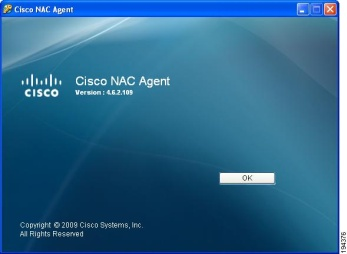
\includegraphics[scale=2]{Figuras/capa-cisco}
	\caption{Cisco NAC Agent \cite{CISCO}}
	\label{fig:ccapa-cisco}
\end{figure}

NAC (Network � uma das op��es tecnol�gicas dispon�veis para a verifica��o e atualiza��o dos sistemas antes de seu ingresso efetivo na rede. � um sistema de controle de acesso � rede com funcionalidades para:
\begin{itemize}
	\item[$\bullet$]Integrar a autentica��o do usu�rio;
	\item[$\bullet$]Gerenciar o acesso �s informa��es da rede;
	\item[$\bullet$]Gerenciar a ``sa�de'' da m�quina com prote��o contra amea�as;
	\item[$\bullet$]Controle de acesso baseado nas pol�ticas da rede da organiza��o;
\end{itemize}

\subsubsection{Autentica��o}
Autentica��o � usada para verificar uma identidade alegada junto � rede para que o acesso seja liberado ou negado.

\subsubsection{Autoriza��o}
Conceito de associar diferentes servi�os aos usu�rios ap�s a autentica��o.

\subsubsection{Valida��o}
� verificado se est� de acordo com as pol�ticas estabelecidas pelo departamento de TI e se atende aos requisitos de verifica��o de patches atualizados, assinaturas de antiv�rus, servi�os e aplica��es ativas.

\subsubsection{Quarentena (Depende da pol�tica do NAC)}
Quando o dispositivo n�o est� em conformidade com as pol�ticas da organiza��o o acesso � rede � bloqueado ou vai para reparo.

\subsubsection{Reparo}
Se o controle de acesso � rede � robusto, ap�s ser redirecionado para um servidor de quarentena, o computador cliente passar� por um reparo de acordo com as pol�ticas pr�-definidas:
\begin{itemize}
	\item[$\bullet$]Atualiza��o das assinaturas de antiv�rus;
	\item[$\bullet$]Atualiza��o dos patches do sistema operacional;
	\item[$\bullet$]Limpeza de malwares detectados;
	\item[$\bullet$]Desativa��o de servi�os desnecess�rios.
\end{itemize}

A inspe��o � uma das principais fun��es da arquitetura NAC e a avalia��o ocorre de acordo com a efici�ncia do sistema de preven��o de intrus�o (IDS/IPS) adotado.

\subsubsection{Servidor Cisco NAC}

\begin{figure}[htp]
	\centering
	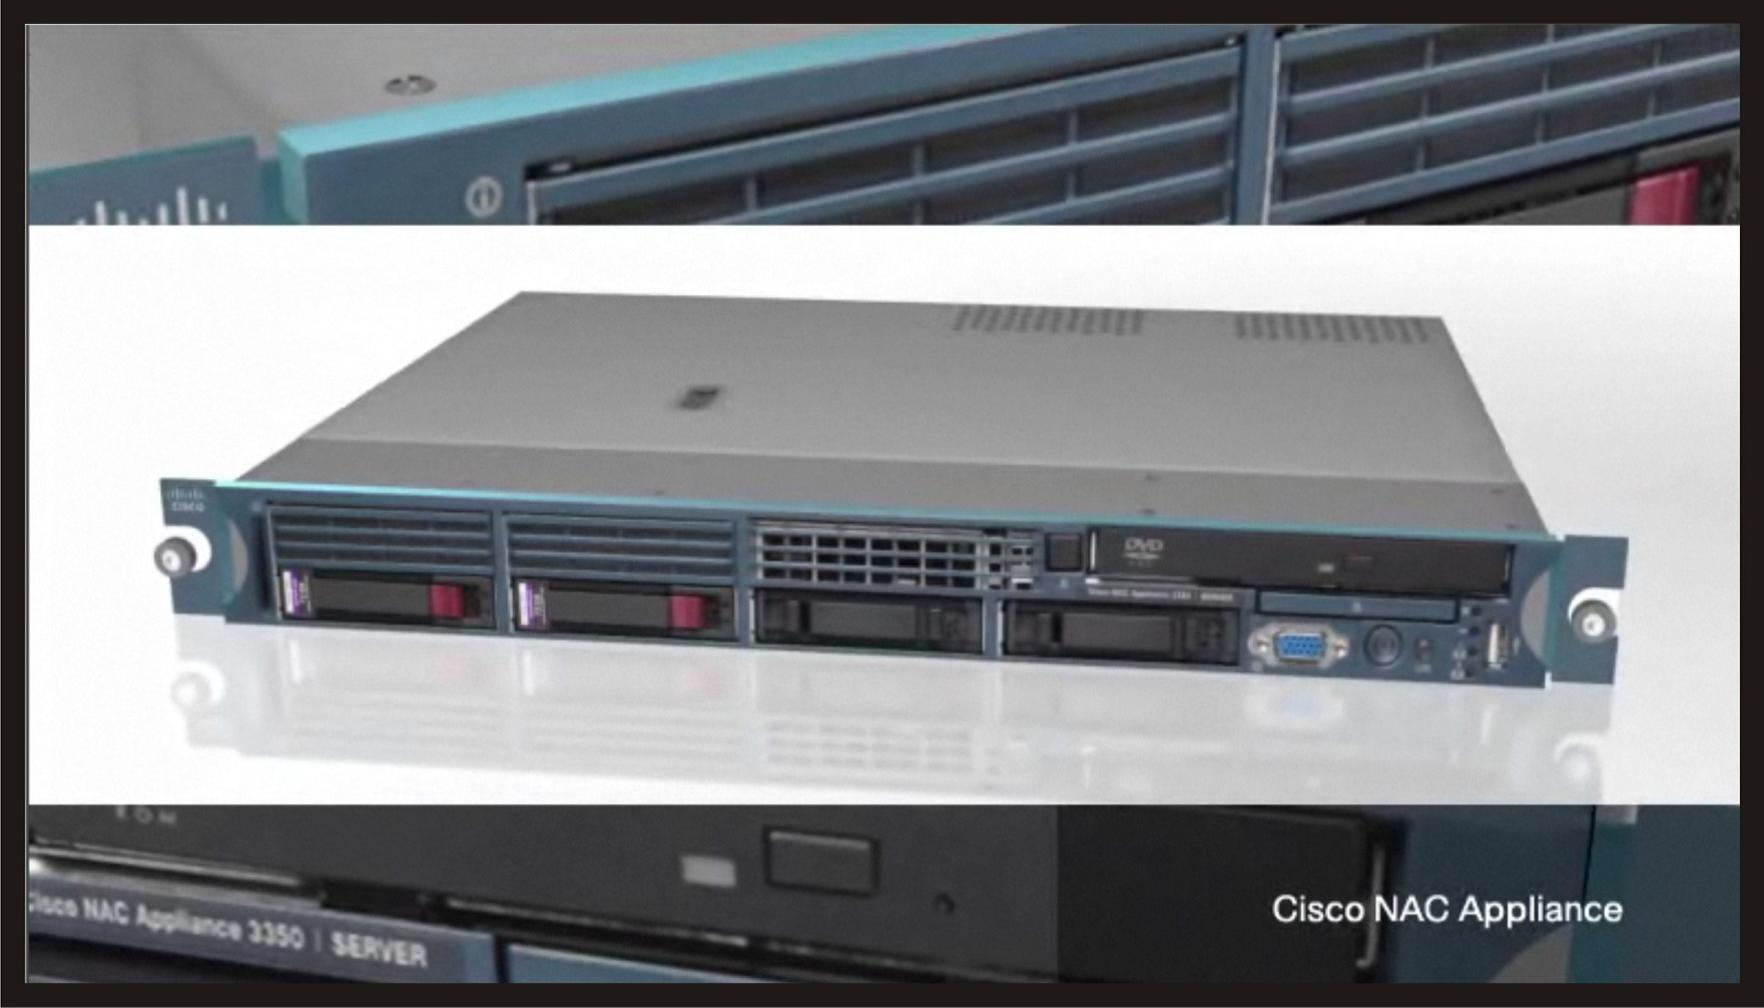
\includegraphics[scale=0.2]{Figuras/servidor-cisco-nac}
	\caption{Servidor Cisco NAC \cite{CISCO}}
	\label{fig:servidor-cisco-nac}
\end{figure}

\subsubsection{Como NAC Funciona}

A figura abaixo representa o funcionamento da NAC \cite{NACAG}.

\begin{figure}[htp]
	\centering
	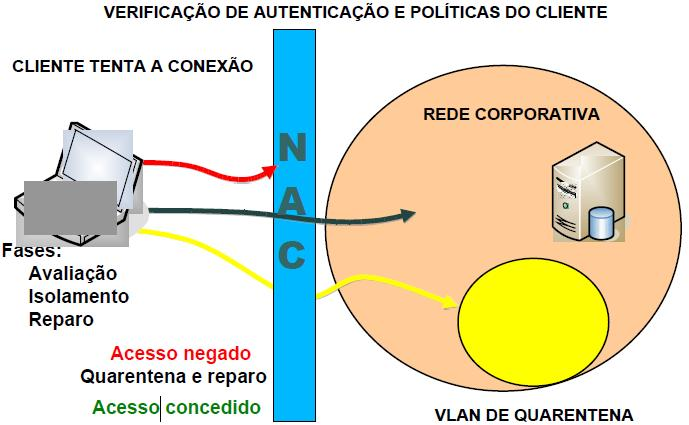
\includegraphics[scale=0.5]{Figuras/funcionamento-nac-cisco}
	\caption{Funcionamento do Cisco NAC \cite{NACI} }
	\label{fig:funcionamento-nac-cisco}
\end{figure}

\subsubsection{Desvantagens}

A rede coorporativa deve estar sempre bem estruturado com o servidor e alinhado informa��es com os analistas dos servidores pois qualquer descuido pode ocasionar lentid�o extrema da rede e impossibilitar acessos de usu�rios no qual est�o ativos. 

\subsection{Check Point}

\begin{figure}[htp]
	\centering
	
\includegraphics[scale=2]{Figuras/capa-checkpoint}
	\caption{Check Point \cite{CHECKPOINT1} }
	\label{fig:capa-checkpoint}
\end{figure}

Check Point  oferece vers�o Media Encryption e Protector Client que protege os dados confidenciais criptografando todas as informa��es dos equipamentos como notebooks e desktops coorporativos bloqueando invas�o de malvaware ou preven��o de c�pia de qualquer informa��o contida no equipamento. Al�m de criptografar m�dia de HD Hard Disc (disco r�gido), Check Point  bloqueia acessos como dispositivos de armazenamento USB, CDs e DVDs e controlar a atividade (ler, escrever e executar) nas portas e dispositivos. Todo o conte�do do dispositivo � automaticamente codificado em segundo plano para uma experi�ncia transparente ao usu�rio final.

A criptografia Check Point Full Disk Encryption simplifica a implementa��o e gerenciamento de seguran�a de endpoint ao criptografar automaticamente todo o conte�do do disco r�gido, inclusive o sistema operacional e arquivos de sistema existentes, tempor�rios e apagados. Este novo n�vel de prote��o protege as empresas de acesso n�o autorizado a informa��es corporativas ou ataques de rede, mesmo se o disco r�gido for fisicamente transferido para outro computador. Possibilita aos clientes protegerem diversos sistemas operacionais, aperfei�oando significativamente a implementa��o e uso de criptografia de disco completo em ambientes mistos. O Check Point Full Disk Encryption tamb�m oferece recursos centralizados de implementa��o, gerenciamento e registro de eventos (logging), para simplificar a administra��o de pol�ticas de seguran�a, dinamizar a conformidade e reduzir o custo total de propriedade. O Check Point Full Disk Encryption � adapt�vel para qualquer organiza��o e foi testado em implementa��es em grandes ind�strias e reparti��es p�blicas em todo o mundo. Al�m disso, o Check Point Full Disk Encryption foi premiado com as mais importantes certifica��es de seguran�a - inclusive International Common Criteria EAL4, FIPS-140-2 e BITS - possibilitando assim r�pida conformidade com regras e regulamenta��es globais de privacidade de dados. N�o importa que sistemas operacionais estejam em uso nas suas redes, os clientes beneficiam-se de tecnologia poderosa de criptografia e seguran�a de dados da Check Point. A estabilidade e flexibilidade do Check Point Full Disk Encryption s�o benef�cios essenciais para gerenciar facilmente nosso ambiente de trabalho sem comprometer o n�vel de seguran�a no endpoint para qualquer sistema operacional em funcionamento \cite{CHECKPOINT2}. 

Podemos agora compartilhar informa��es sem dificuldades, sabendo que os dados de nossos clientes est�o seguros.

\begin{itemize}
	\item[$\bullet$]Autentica��o Pr�-Inicializa��o que requer nome de usu�rio e senha antes que o sistema operacional seja carregado, elevando a seguran�a. O Check Point Full Disk Encryption tamb�m permite autentica��o multifatores, como Smart Cards ou tokens baseados em certifica��es;
	\item[$\bullet$]Ajuda Segura Remota d� aos usu�rios op��es de ajuda remota e suporte remoto baseado na web para tokens e senhas de acesso perdidos;
	\item[$\bullet$]A Interface �nica de Usu�rio simplifica a instala��o, administra��o e f�cil integra��o, suporta diversas linguagem para implementa��es globais. A opera��o autom�tica e transparente tem efeito m�nimo sobre a produtividade dos usu�rios finais; e
	\item[$\bullet$]Gerenciamento Central e Registro de Eventos permitem fiscaliza��o central de pol�ticas de seguran�as para atender as crescentes necessidades de conformidade. O gerenciamento central de configura��o reduz o custo total de propriedade.Nota: As informa��es foram fornecidas pela Check Point.
\end{itemize}

\subsubsection{Desvantagens}

Dependendo da quantidade de informa��es o processo de criptografia pode ser demorado.

O equipamento apresentando problemas no sistema operacional ao efetuar o backup o analista deve conter em m�os o CD de descriptografia caso contr�rio o mesmo deve solicitar ao suporte checkpoint o CD no qual esse processo � um pouco demorado e burocr�tico.

\subsection{Outras Ferramentas}

\subsubsection{OTP (One Time Password)}
Ferramenta composta de senha de uso �nico. Utiliza complexos algoritmos criptogr�ficos unidirecionais com base em um n�mero aleat�rio. 
``Uma forma de identifica��o do usu�rio em determinados ambientes. A solu��o tem tr�s modalidades difundidas: sincronismo por evento - senhas geradas a partir de uma fun��o recursiva que utiliza a semente e o �ltimo n�mero gerado; por tempo - sincroniza��o ente dispositivo e servidor; ou desafios/respostas onde a senha � gerada com base na semente e um desafio (n�mero) informado pelo servidor.'' (Julio Graziano Pontes - Gerente de Servi�os da True Access)

\subsubsection{CPQD (Gest�o Integrada de Fraudes e Eventos)}
Voltada para a preven��o de fraudes em transa��es banc�rias, apoia a monitora��o e a investiga��o on-line e em tempo real, de forma pr�-ativa, de transa��es monet�rias e n�o monet�rias realizadas por meio dos diversos canais de relacionamento. A solu��o do CPqD promove uma completa integra��o entre: core  banc�rio (autorizadores), eventos e incidentes de seguran�a e o tratamento de transa��es suspeitas.

\subsubsection{ACI Proactive Risk Manager \cite{ACIPAYMENT}}
Solu��o abrangente de gerenciamento de crime financeiro, uma solu��o para auxiliar emissores de cart�es, comerciantes e compradores a combater a fraude das institui��es financeiras e esquemas de lavagem de dinheiro.

\begin{figure}[htp]
	\centering
	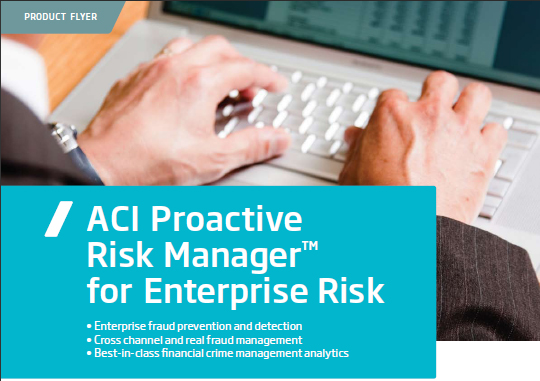
\includegraphics[scale=0.5]{Figuras/ferramentas-ACI-Proactive}
	\caption{Proactive Risk Manager for Enterprise Risk}
	\label{fig:ferramentas-ACI-Proactive}
\end{figure}

\subsubsection{CanIt AntiSpam \cite{CANITANTISPAM}}
O CanIt � uma poderosa ferramenta de combate a spam, v�rus e fraudes eletr�nicas utilizado por importantes empresas brasileiras. Dentre os clientes, destacam-se in�meros provedores de internet como America-Net, Netlink, BitcomNet, diversas  institui��es de ensino como Universidade de Bras�lia, FMU, Universidade Federal de Pernambuco, UFPE, Universidade Federal de Vi�osa, Universidade Federal de Itajub�, Unesp, al�m de TV Cultura, Berkley International, entre outras. Compat�vel com sistemas Microsoft Exchange, Lotus Notes, Linux Based, atende a corpora��es desde 5 at� milh�es de caixas postais.
\pagebreak
\begin{figure}[htp]
	\centering
	
\includegraphics[scale=1]{Figuras/ferramentas-canit-antispam}
	\caption{CanIt AntiSpam}
	\label{fig:ferramentas-canit-antispam}
\end{figure}
% \chapter{Roadmap de produtos, vers�es, etc...}
\chapter{Case de sucesso}

\section{OTP (One Time Password) com integra��o ao Connectra da Check Point}

A implementa��o da ferramenta em conjunto assegurou uma seguran�a maior e resultou na redu��o � quase zero da incid�ncia de fraudes.

A companhia implementou essa ferramenta em uma rede de loja varejista que comercializava seus produtos e servi�os atrav�s de canais de venda distribu�dos pelo Brasil. Os sistemas de frente de caixa e retaguarda eram disponibilizados aos canais pela web, o que havia alto �ndice de fraudes. ``O grande problema nesse caso era o compartilhamento de senhas e a gest�o desse ambiente''. 

``Foi usada a integra��o do Connectra com o OTP para proporcionar autentica��o segura com custo baixo. Tamb�m foi implementado um sistema de gest�o de identidades para sincronizar os contratos do lojista e conceder os acessos em tempo real. 

Nosso cliente tem acesso a uma p�gina na web onde est�o os aplicativos e essa pagina baixa um script que verifica a seguran�a da esta��o. Em um segundo momento, o usu�rio envia as credenciais (conta e senha) mais a OTP, onde � garantida a seguran�a de quem est� acessando estabelecendo um canal seguro. Com o OTP conseguimos integrar as aplica��es com efeito na execu��o e combate a fraudes, roubo de senhas foram evitados nesse processo'' (Julio Graziano Pontes - Gerente de Servi�os da True Access)

% \chapter{Vantagens e Desvantagens}
% \chapter{Concorrentes}
\chapter{Recupera��o de Perdas}

\section{Impacto de Fraudes Financeiras}
Para \cite[p.~04]{FRAUELE}, a fraude eletr�nica � um grande desafio para o setor financeiro.

\begin{citacao}
Segundo \cite[p.~02]{CAMARGO} a auditoria de sistemas em ``e-business'' e fraudes eletr�nicas � um dos maiores desafios da fiscaliza��o do sistema financeiro. O aumento substancial das negocia��es via internet, conforme destacado pela pesquisa da Federa��o Brasileira dos Bancos (FEBRABAN), segundo a qual as transa��es por ``internet banking P.F.'' cresceram 450\% entre 2000 e 2004, � a maior causa do crescimento deste tipo de auditoria. A instantaneidade dessas negocia��es via cart�o de cr�dito impacta em maiores riscos de fraudes, pois muitas das vezes tais negocia��es s�o autorizadas sem a efetiva participa��o, ou seja, presen�a do cliente.
\end{citacao}

Atualmente, Eduardo Chedid, vice-presidente executivo de produtos e neg�cios da Cielo, a cada R\$ 100 gastos em compras, R\$ 0,75 (figura \ref{fig:estatisticas-fraudes-cartoes} s�o fraudados \cite{FRAUDECARTAOCIELO}, ou seja, a realidade apresentada em 2007 por \cite{FRAUELE} continua presente.

\begin{figure}[htp]
  \centering
  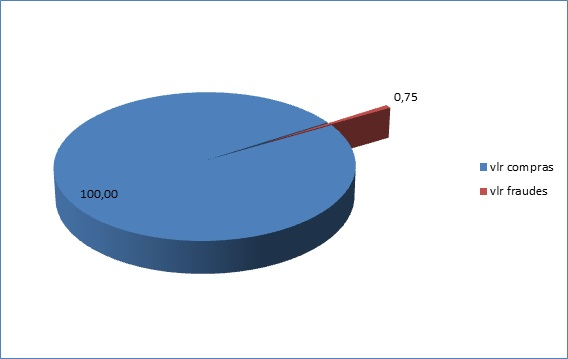
\includegraphics[scale=0.6]{Figuras/estatisticas-fraudes-cartoes}
  \caption{Fraudes em Transa��es Eletr�nicas}
  \label{fig:estatisticas-fraudes-cartoes}
\end{figure}

O Brasil movimentou mais de 670 bilh�es de reais em transa��es de cart�es (opera��es de d�bito e cr�dito) em 2011 \cite{ESTADAO}. Isso representa mais de 5 bilh�es de reais seriam desprendidos somente com fraudes eletr�nicas.

Em pesquisa do Norton \cite{NORTON} o e-crime chega a movimentar mais de  US\$114 bilh�es e as empresas gastam mais cerca de US\$274 bilh�es com repara��es, juntos somam US\$388 bilh�es de prejuizos no total.

Dados apontam que o crime tradicional est� migrando em grande escala para o mundo virtual, segundo noticia da Adrenaline \cite{ADCC}:

\begin{citacao}
Em 2010, foram R\$900 milh�es roubados atrav�s de golpes online, contra ``s�'' R\$55 milh�es do crime tradicional. E a tend�ncia � de aumentar, e muito: apenas na primeira metade deste ano, foram R\$685 milh�es desviados via Internet.
\end{citacao}

Em pesquisa da Symantec \cite{SYMANTECREL2011}, al�m do impacto financeiro o roubo de informa��es pessoais gerou um dos maiores impactos com perdas sofridas pelo cibercrime.

\begin{figure}[htp]
  \centering
  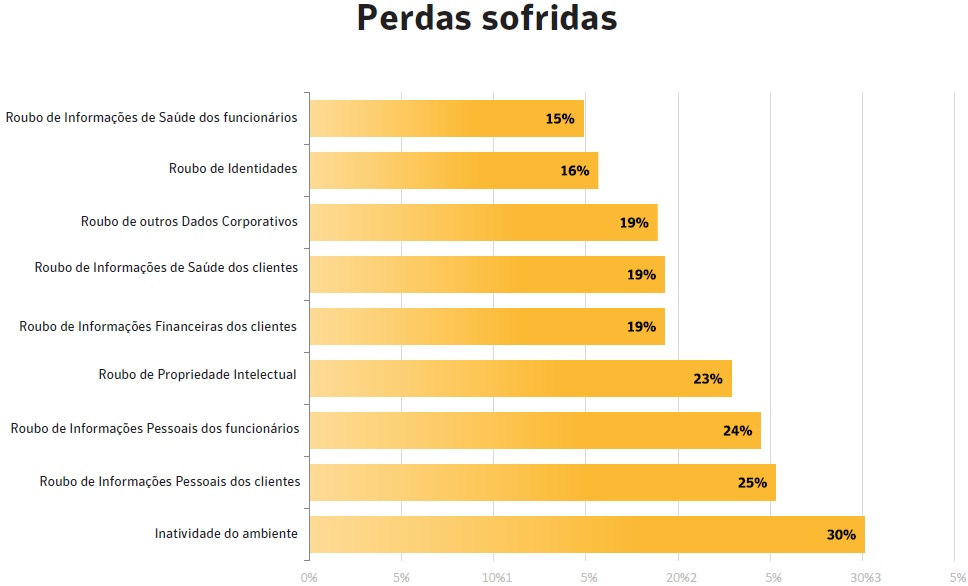
\includegraphics[scale=0.5]{Figuras/perdas-sofridas}
  \caption{Perdas sofridas\cite{SYMANTECREL2011}}
  \label{fig:perdas-sofridas}
\end{figure}

\begin{figure}[htp]
  \centering
  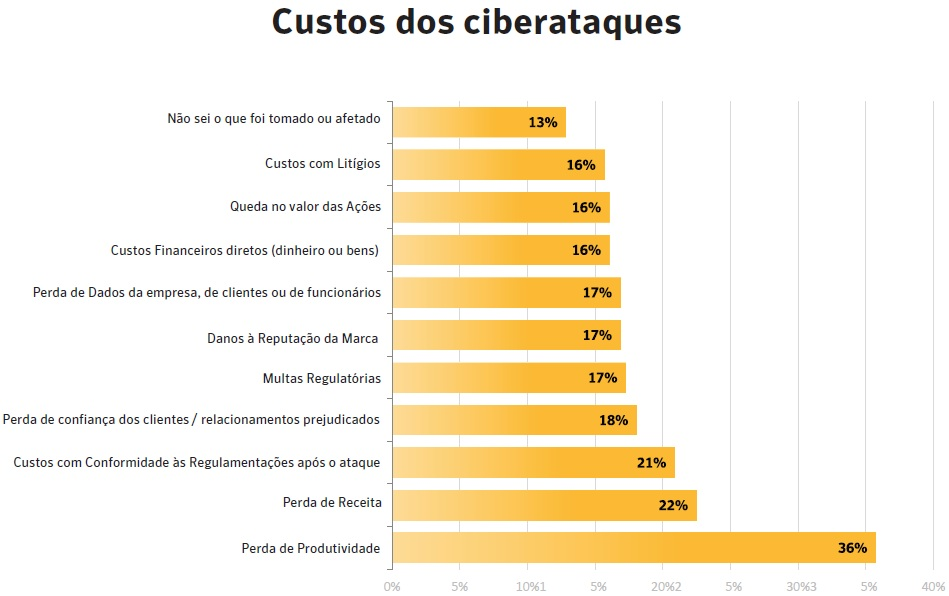
\includegraphics[scale=0.5]{Figuras/custos-dos-ciberataques}
  \caption{Custos do ciberataque\cite{SYMANTECREL2011}}
  \label{fig:custos-dos-ciberataques}
\end{figure}

\section{C�lculo das Chances de Recupera��o de Perdas}

Question�rio de probabil�stico de recupera��o de perdas com fraudes. � um servi�o que visa estimar a probabilidade de se recuperar uma parte consistente das perdas. Tamb�m estima a oportunidade de iniciar uma a��o de recupera��o atrav�s de uma empresa de recupera��o de perdas por fraudes. Obviamente, o servi�o � indicativo, sendo necess�ria uma an�lise mais profunda em cada caso para se obter um parecer mais confi�vel. 

\section{Procedimentos para Recupera��o de Perdas}

A recupera��o de perdas por uma empresa � um processo quase sempre problem�tico. Por tal motivo deve ser administrado por especialistas. Muitos golpes apresentam tra�os comuns dos criminosos, a preocupa��o em ocultar sua verdadeira identidade, rapidez e efici�ncia em desaparecer com os bens furtados.

\begin{figure}[htp]
  \centering
  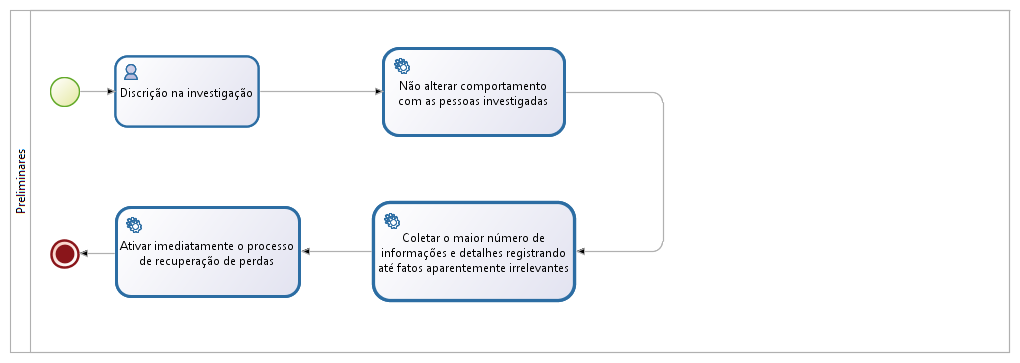
\includegraphics[scale=0.5]{Figuras/proc-recupera-preliminar01}
  \caption{Preliminares ao Processo de Recupera��o}
  \label{fig:proc-recupera-preliminar01}
\end{figure}

\begin{figure}[htp]
  \centering
  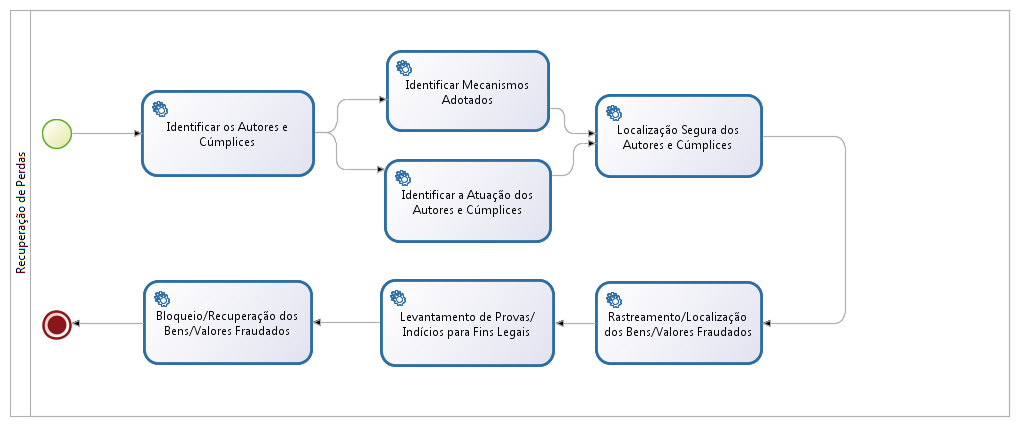
\includegraphics[scale=0.75, angle=90]{Figuras/proc-recupera01}
  \caption{Processo de Recupera��o}
  \label{fig:proc-recupera01}
\end{figure}

\chapter{Conclus�o}

Como podemos ver ao longo do documento o cibercrime\footnote{� todo crime onde o computador � o principal meio para comet�-lo} tem diversas facetas e muda constantemente. Dentro deste, a fraude � um dos principais crimes cometidos e tem como maior vetor o phishing, inclusive foi apresentado um caso recente que chamou a aten��o da m�dia recentemente \footnote{Caso Carolina Dieckmann}.

Nesse problema mundial de fraudes, o Brasil se destaca negativamente ao liderar o \emph{ranking} dos maiores produtores e utilizadores de \emph{banker} do mundo e que ao contr�rio do que se possa esperar a maioria dos ataques feitos s�o realizados por pessoas com pouco conhecimento t�cnico que se utilizam de \emph{receitas de bolos\footnote{C�digos maliciosos de terceiros}} para a pr�tica do il�cito.

Podemos analisar a estrutura atual do crime organizado e como o processo funciona aliciando laranjas para mascarar o dinheiro furtado. Analisamos quest�es legais e chegamos a discurs�o sobre preven��o e combate ao cibercrime em diversos aspectos e seus novos desafios. Mostramos a rea��o do mercado com seus produtos e solu��es comerciais. Por fim mostramos o estrago que o cibercrime causa na economia.
% referencias

\href{http://www.fraudes.org/recupera.asp}{Perdas e Recupera��o}
\href{http://mariano.delegadodepolicia.com/tag/pcc}{Pesquisar crime organizado brasileiro ligado ao cibercrime}

% legisla��o
% ISO: http://www.27000.org
% Paper do Coriolano: http://www2.oabsp.org.br/asp/comissoes/sociedade_informacao/artigos/crimes_ciberneticos.pdf
% Projeto de Lei 2126/2011: http://www.camara.gov.br/proposicoesWeb/fichadetramitacao?idProposicao=517255
% PCC e CV: http://mariano.delegadodepolicia.com/tag/pcc
% Marco civil: http://culturadigital.br/marcocivil/2011/10/27/marco-civil-encaminhado-ao-congress/


\href{http://icommercepage.wordpress.com/2009/07/12/classificacao-dos-crimes-digitais/}
\href{http://convergenciadigital.uol.com.br/cgi/cgilua.exe/sys/start.htm?infoid=16378\&sid=17}
\href{http://pingado.terra.com.br/noticias/57825/tecn-da-informacao/antonio-gesteira-presidente-da-nfe-do-brasil-preve-aumento-da-fiscalizacao-da-receita-fe.html}
\href{http://www1.folha.uol.com.br/folha/informatica/ult124u19455.shtml}{Juliana Carpanez - Folha Online}
\href{http://cartilha.cert.br/fraudes/}
\href{http://www.fraudes.org/}
\href{http://www.valorizeseudinheiro.com.br/dicas-para-evitar-fraudes-em-cheques/}
\href{http://forensedigital.com.br/new/o-mercado-negro-do-cibercrime-em-expansao/}
\href{http://www.fbi.gov/about-us/investigate/cyber/cyber}
\href{http://www.ic3.gov/default.aspx}
\href{http://www.tecmundo.com.br/conexao/3486-conheca-os-cybercrimes-e-aprenda-a-se-defender-deles.htm}
\href{http://mariano.delegadodepolicia.com/category/artigos/}
\href{http://www.nytimes.com/2003/10/27/business/technology-brazil-becomes-a-cybercrime-lab.html?pagewanted=all&src=pm}
\href{http://nakedsecurity.sophos.com/2011/10/05/brazils-cybercrime-evolution-it-doesnt-look-pretty/}
\href{http://idgnow.uol.com.br/internet/2007/05/11/idgnoticia.2007-05-10.5490328067/paginador/pagina_5}
\href{http://www.fraudeseletronicas.com.br/}
\href{http://jus.com.br/revista/texto/2250/crimes-de-informatica}
% \href{http://imasters.com.br/artigo/9741/forense/google_forensics_investigando_cybercrimes}
\href{http://forensedigital.com.br/new/o-mercado-negro-do-cibercrime-em-expansao/}
\href{http://itweb.com.br/53372/orgaos-legais-detectam-5-vezes-mais-casos-de-cibercrime-em-2011/}
\href{http://www.slideshare.net/fullscreen/Trustwave/executive-summary-trustwave-2012-global-security-report/1}


MODUS OPERANDI

\href{http://www.drtomoconnor.com/3100/3100lect04.htm}{}


ESTAT�STICA

\href{http://www.crimecibernetico.com.br/} {}
% \href{http://www.relatoriobancario.com.br/rb/noticias/cielo_fecha_parceria_para_prevencao_de_fraudes_eletronicas}{}

COMBATE

\href{http://olhardigital.uol.com.br/negocios/digital_news/noticias/lei_de_crimes_na_internet_entenda_as_principais_polemicas_em_torno_do_projeto}
\href{http://www.cmsoftware.com.br/produto-neural-risk-persona-fraud-free.asp}
\href{http://olhardigital.uol.com.br/negocios/digital_news/noticias/fraudes_eletronicas_bancarias_geraram_perdas_de_r_685_milhoes_no_semestre}
\href{http://www.rac.com.br/institucionais/cenario-xxi/2005/02/26/3193/cpqd-e-cerebrus-se-aliam-contra-fraudadores}{}

FRAUDES

\href{http://www.decisionreport.com.br/publique/cgi/cgilua.exe/sys/start.htm?infoid=8136&sid=42}{}

PERDAS FINANCEIRAS

\href{http://www.febraban.org.br/Noticias1.asp?id_texto=1321}{}

CEN�RIO ATUAL

\href{http://www2.oabsp.org.br/asp/comissoes/sociedade_informacao/artigos/crimes_ciberneticos.pdf}{}


FILMES RECOMENDADOS

\begin{itemize}
  \item[$\bullet$]Catch Me If You Can (2002) ? [Prenda-me se for capaz]
  \item[$\bullet$]Fun with Dick and Jane ? [Jick \& Jane]
  \item[$\bullet$]Trakedown - [Filme sobre o Mitnik]
\end{itemize}

% % \chapter{Gloss�rio}
% 
% Wares: visam a quebra de prote��o de programas originais. Seus alvos s�o os sharewares (programas demonstrativos com prazo de utiliza��o);
% 
% Phreaker: visam as centrais telef�nicas, executando liga��es clandestinas, liga��es internacionais. Normalmente formados pelas pr�prias empresas de telefonia (funcion�rio demitido, insatisfeito, etc.);
% 
% Lammers: consideram-se hackers, gostam de aparecer, normalmente discriminam os novatos (eles mesmos). Agem na sua grande maioria utilizando scripts encontrados na web.
% 
% Roubo de Identidade: 
% 
% Pedofilia: 
% 
% Cal�nia e Difama��o: .
% 
% Amea�a: 	.
% 
% Discrimina��o: 		.
% Espionagem Industrial: .
% 
% % \printglossary

\bibliography{bb}
\bibliographystyle{abnt-alf}

\end{document}
